\documentclass[aspectratio=169,usepdftitle=true,11pt,ngerman,t]{beamer}

\newcommand\lqfirstname{Name}
\newcommand\lqfullname{Name Last}
\newcommand\lqemail{name.last}
\errorcontextlines999999

% base
\usepackage[utf8]{inputenc}
\usepackage[T1]{fontenc}
\usepackage{lmodern}
\usepackage{microtype}
\usepackage[main=ngerman]{babel}
\usepackage{csquotes}

% graphics
\usepackage[prefix=]{xcolor-material}
\usepackage{graphics}
\usepackage{tcolorbox}
\usepackage{twemojis}
\usepackage{tikz}
\usetikzlibrary{
    positioning,
    calc,
    tikzmark,
    circuits.logic.IEC
}

% math
\usepackage{amsmath,amssymb}
\usepackage{mathtools}
\usepackage{array}
\usepackage{booktabs}
\usepackage{cancel}
\usepackage{ulem}

% flo
\usepackage{fancyqr}
\usepackage[addons]{color-palettes}
\usepackage[encoding,noloadlangs,cpalette,numinpar,fakeminted]{sopra-listings}
\usepackage{code-animation}
\usetheme[theorems]{colorful-dream}
\theoremstyle{exercise}
\newtheorem*{exercise*}{Aufgabe}
\theoremstyle{solve}
\newtheorem*{solve*}{Lösung}

% tools
\usepackage{algpseudocode}
\usepackage{dirtree}

% warnings
\usepackage{silence}
\WarningFilter{latexfont}{Some font shapes were not available}
\WarningFilter{latexfont}{Font shape}
\WarningFilter{pgf}{Returning node center instead of a point on node border}
\let\origenddocument\enddocument\renewcommand{\enddocument}{\hfuzz=10.95pt\origenddocument}
% title image: box
% ([vshift], inverse scale, width, content)
\newcommand\titleimagebox[4][0pt]{%
\newlength\tibheight\setlength\tibheight{4cm}
\newlength\tibtY\setlength\tibtY{-6em}
\titleimage{\begin{minipage}[c][#2\tibheight]{#3}\vspace*{#2\tibtY}%
    \vspace*{#1}\begin{tcolorbox}[boxrule=0.1pt]%
    \centering#4% TODO: bug: not centered if too wide
    \end{tcolorbox}%
\end{minipage}}}

% outro image: text
% (text)
\newcommand\outroimagetext[1]{\outro{Karlsruhe, \today%
\begin{tikzpicture}[remember picture,overlay]
    \node[align=center] at (current page.center) {#1};
\end{tikzpicture}}}% chktex 31

% reset counters
\newcommand\resetframecounters{\addtocounter{exercise}{-1}\addtocounter{solve}{-1}}
\newcommand\resetex{\addtocounter{exercise}{-1}}
\newcommand\resetsolve{\addtocounter{solve}{-1}}

% small footnote
\newcommand{\nicefootnote}[1]{\tikz[overlay,remember picture]{\node[anchor=south,text width=\dimexpr\textwidth+2em\relax,align=center,above=1em of current page.south] (nicefootnote) {\hrule\vspace{1pt}\footnotesize#1};}}

% kv
% ([draw], variables, values)
% {currently only works correctly for 4 variables}
\newcommand{\lqkv}[3][]{
    \begin{tikzpicture}
        \foreach \v [count=\k from 1] in {#2} {\global\let\Vdim=\k}
        \pgfmathsetmacro\rows{2^ceil(\Vdim/2)}
        \pgfmathsetmacro\cols{2^int(\Vdim/2)}

        \foreach \v [count=\k from 1] in {#2} {
            \pgfmathsetmacro\shift{0.5+floor(\k*ceil(\Vdim/2)/2)}

            \ifcase\k\relax
            \or
                \draw (\shift-1,0.75) -- (\shift+1,0.75);
                \node[fill=white] at (\shift,0.75) {\v};
            \or
                \draw (-0.75,-\shift) -- (-0.75,-\shift+2);
                \node[fill=white] at (-0.75,-\shift+1) {\v};
            \or
                \draw (\shift-2,-\cols+0.25) -- (\shift,-\cols+0.25);
                \node[fill=white] at (\shift-1,-\cols+0.25) {\v};
            \or
                \draw (\cols-0.25,-\shift+1) -- (\cols-0.25,-\shift+3);
                \node[fill=white] at (\cols-0.25,-\shift+2) {\v};
            \fi
        }
      
        \foreach \v [count=\k from 0] in {#3} {
            \pgfmathsetmacro\x{mod(\k,\rows)}
            \pgfmathsetmacro\y{int(\k/\rows)}
            \node[draw, minimum width=1cm, minimum height=1cm, align=center] at (\x,-\y) {\v};
        }

        \begin{scope}
            \clip (-0.5,0.5) rectangle (3.5,-3.5);
            \foreach \r in {#1} {\draw[rounded corners=1ex] \r;}
        \end{scope}

        \global\let\Vdim\undefined
    \end{tikzpicture}
}
\title{Digitaltechnik}
\institute{Karlsruher Institut für Technologie}

\author{\lqfullname}
\email{\lqemail @student.kit.edu}% chktex 1
% credit flo
\addtobeamertemplate{title page}{}{%
\scriptsize\color{gray}\begin{tikzpicture}[overlay, remember picture]
    \node[above left = 1em and 1em of current page.south east,align=center] (n0) {\LaTeX-Vorlage von\\\href{https://github.com/EagleoutIce}{Florian Sihler}};
    \node[above = 0cm of n0] (n1) {\fancyqr[size=1.5cm,tight]{https://eagleoutice.github.io/beamer-themes/\#colorful-dream}};
\end{tikzpicture}}% chktex 31

%%%%%%%%%%%%%%%%%%%%%%%%%%%%%%%%%%%%%%%%%%%%%%%%%%%%%%%%%%%%%%%%

\subtitle{Tutorium 1}
\date{12. Mai 2026}

\titleimagebox{1}{8cm}{
    \textbf{\color{red}Breaking News:} new PB of 2:00
    \onslide<2>\\\textit{Spoiler: Das ist nicht viel Zeit \texttwemoji{sob}}
}

\outroimagetext{\large\textbf{42 69 73 20 6E E4 63 68 73 74 65 20 57 6F 63 68 65 20 3A 29}}

%%%%%%%%%%%%%%%%%%%%%%%%%%%%%%%%%%%%%%%%%%%%%%%%%%%%%%%%%%%%%%%%

\title{Digitaltechnik}

\begin{document}

\section*{Folien}
\begin{frame}{now 4 real}\onslide<+->
    \begin{block}{\faGithub~Laqco}
        \begin{minipage}{0.75\linewidth}
            Jetzt sind die Folien auch wirklich hochgeladen!
            \vspace{\baselineskip}\\
            \textit{Warum ist das mittig? Ich weiß es nicht.~\alt<+->{\texttwemoji{frowning}}{:D}}
        \end{minipage}\nolinebreak\hfill\begin{minipage}{0.25\linewidth}
            \vspace{0.107cm}\fancyqr[size=3.5cm,color=black!90!gray]{https://github.com/Laqco/kit-dt-ss26/tree/builds/pdfs}
        \end{minipage}
    \end{block}\onslide<+->
    \begin{itemize}
        \item Lösungen von euch?
    \end{itemize}
\end{frame}

\section[Von Zahlen und Buchstaben\dots
\\\small Oder: Als ob ich schon korrigiert hätte \texttwemoji{joy}]{Übungsblatt 1}

\subsection{Aufgabe 2}
\begin{frame}{Aufgabe 1\dots?}\onslide<+->
    \begin{exercise}
        Stellen Sie den Text \enquote{Ist das schwierig?} im ASCII-Format als Dezimal-, Binär- und Hexadezimalzahlen dar.
    \end{exercise}
    \begin{solve}[Laaaaaangweilig \texttwemoji{roll_eyes}]
        \onslide<+->\begin{tikzpicture}[overlay]
            \node[align=left,below left=2cm of current page.east] {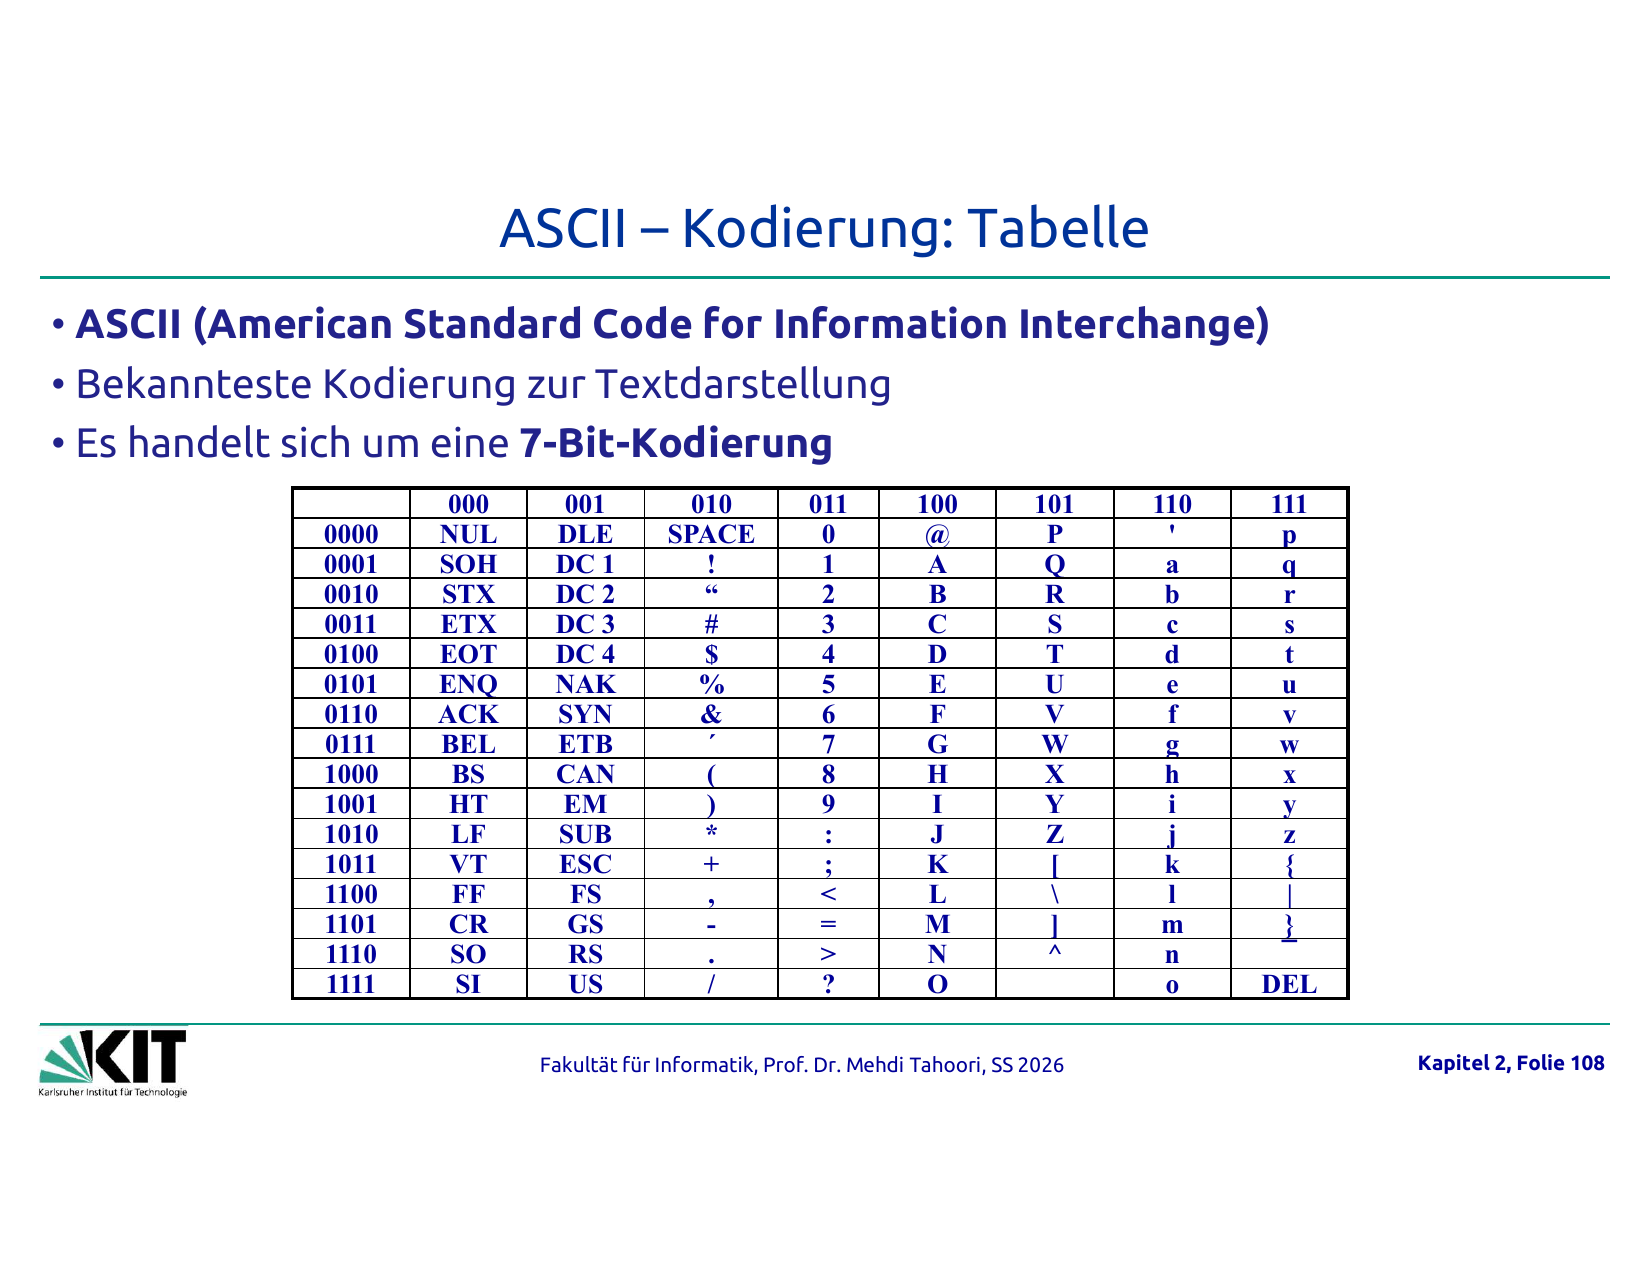
\includegraphics[scale=0.2]{slide12.png}};
        \end{tikzpicture}
        \vspace*{-\baselineskip}
        \begin{itemize}
            \item \(1001001\onslide<+->~1110011\onslide<+->~1110100\onslide<+->~\alt<.>{\mathbf{0}}{0}100000\onslide<+->~\dots \)
            \item \(0x49~0x73~0x74~0x20~\dots \)% chktex 29
            \item \(73~115~116~32~\dots \)
        \end{itemize}
    \end{solve}
\end{frame}
\begin{frame}{Vielleicht geht es ja auch einfacher\dots}
    \begin{exercise}[\enquote{Ist das schwierig?} \faAngleRight~ASCII (Dec, Bin, Hex)]\end{exercise}
    \begin{solve}[Trickserei!]
        Schauen wir uns das mal genauer an:
        \begin{itemize}
            \item<2-> \(\mathtt{'a'}={\only<6->{\color{purple}}011}0~0001_{(2)}=97_{(10)}\)
            \item<4-> \(\mathtt{'b'}={\only<6->{\color{purple}}011}0~0010_{(2)}=98_{(10)}\)
            \item<6-> \(\cdots \)
            \item<3-> \(\mathtt{'A'}={\only<6->{\color{purple}}010}0~0001_{(2)}=65_{(10)}\)
            \item<5-> \(\mathtt{'B'}={\only<6->{\color{purple}}0\tikzmark{binmark0}10}0~0010_{(2)}=66_{(10)}\)
            \item<6-> \(\cdots \)
        \end{itemize}
    \end{solve}
    \onslide<6->\begin{tikzpicture}[overlay,remember picture]
        \node [inner sep=0,below right = 0.05cm and 2pt of pic cs:binmark0] (n0) {};
        \node [inner sep=2pt,below right = 0em and 12em of pic cs:binmark0,draw=purple,rounded corners] (n1) {\begin{minipage}{0.5\textwidth}
            \centering\scriptsize Da unser Alphabet \(26_{(10)}=11010_{(2)}\) Buchstaben\\hat, müssen wir \(5\) Stellen rechts freihalten!
        \end{minipage}};
        \node [inner sep=0,below left = -0.35cm and 0.05cm of n1] (n2) {};
        \draw (n0) edge[->,bend right=20] (n2);
    \end{tikzpicture}
\end{frame}

\addtocounter{exercise}{-1}\addtocounter{solve}{-1}
\begin{frame}[noframenumbering]{Vielleicht geht es ja auch einfacher\dots}
    \begin{exercise}[\enquote{Ist das schwierig?} \faAngleRight~ASCII (Dec, Bin, Hex)]\end{exercise}
    \begin{solve}[Trickserei!]
        Das heißt:\begin{itemize}
            \item<2-> Kleinbuchstaben: \(\textcolor{purple}{011}0\only<4|handout:0>{\mathllap{\underbrace{\hphantom{0110}}_\text{\color{lightgray}0x\color{blue}6}}}~0001\only<4|handout:0>{\mathllap{\underbrace{\hphantom{0001}}_\text{\color{lightgray}0x\color{blue}1}}}\)~---~\(\textcolor{purple}{011}1\only<4|handout:0>{\mathllap{\underbrace{\hphantom{0111}}_\text{\color{lightgray}0x\color{blue}7}}}~1010\only<4|handout:0>{\mathllap{\underbrace{\hphantom{1010}}_\text{\color{lightgray}0x\color{blue}A}}}\)\only<4|handout:0>{\vspace{-3pt}}\\
            \hphantom{Kleinbuchstaben: }\only<5->{\(\color{lightgray}0x\color{blue}61\)~---~\(\color{lightgray}0x\color{blue}7A\)}\\
            \hphantom{Kleinbuchstaben: }\only<6->{\(97\)~---~\(122\)}
            \item<3-> Großbuchstaben: \(\textcolor{purple}{010}0\only<4|handout:0>{\mathllap{\underbrace{\hphantom{0100}}_\text{\color{lightgray}0x\color{blue}4}}}~0001\only<4|handout:0>{\mathllap{\underbrace{\hphantom{0001}}_\text{\color{lightgray}0x\color{blue}1}}}\)~---~\(\textcolor{purple}{010}1\only<4|handout:0>{\mathllap{\underbrace{\hphantom{0101}}_\text{\color{lightgray}0x\color{blue}5}}}~1010\only<4|handout:0>{\mathllap{\underbrace{\hphantom{1010}}_\text{\color{lightgray}0x\color{blue}A}}}\)\only<4|handout:0>{\vspace{-3pt}}\\
            \hphantom{Großbuchstaben: }\only<5->{\(\color{lightgray}0x\color{blue}41\)~---~\(\color{lightgray}0x\color{blue}5A\)}\\
            \hphantom{Großbuchstaben: }\only<6->{\(65\)~---~\(90\)}
        \end{itemize}
    \end{solve}
\end{frame}

\subsection{Aufgabe 3}
\begin{frame}{Habt ihr euch schonmal gefragt?}\onslide<+->
    \dots warum eine \(32\)-Bit Gleitkommazahl genau einen 8-Bit langen (verschobenen) Exponenten hat?
    \begin{itemize}[<+->]
        \item \href{https://ieeexplore.ieee.org/document/8766229}{IEEE 754 (2019)} definiert für Bitzahl \(\geq 64\): \(w = round(4\times \log_2(k))-13\)\onslide<+->\\
            \(w = round(4\times \log_2(32))-13 = 7 \neq 8\)~???
        \item NASA VAX F benutzte 8 Bit, um physikalische Konstanten darstellen zu können!\nicefootnote{https://retrocomputing.stackexchange.com/questions/13493}
    \end{itemize}
    
    \onslide<+->\dots was ein längerer oder kürzerer Exponent verändert?
    \begin{itemize}
        \item[\faAngleRight]<+-> Aufgabe 3
    \end{itemize}
\end{frame}

\begin{frame}{Der Vergleich}\onslide<+->
    \begin{exercise}Stellen Sie die Zahl \(0,4\) im jeweiligen Format dar und berechnen Sie den relativen Fehler.\end{exercise}
    \begin{solve}
        \onslide<+->Umrechnung: \(0{,}4_{10} = 0{,}0\overline{1100}_2 = 1{,}\overline{1001}_2 \cdot 2^{-2}\)
        \onslide<. (1)->
        \begin{itemize}
            \item \only<+>{\textbf{2-Bit} (Bias~\(=1\)): \(0{,}4 < 1\) (kleinste norm. Zahl) \(\Rightarrow \) Denormzahl.\\
                Mantisse (5~Bit, abgeschnitten): \(0{,}01100_2\) \\
                Bitmuster: \(\texttt{0\,00\,01100}\), Wert: \(0{,}01100_2 = 0{,}375\) \\
                Rel. Fehler: \(\dfrac{|0{,}4 - 0{,}375|}{0{,}4} = 6{,}25\% \)}%
            \only<+>{\textbf{3-Bit} (Bias~\(=3\)): Exponent \(-2 \Rightarrow \) gespeicherter Exponent \(= -2+3 = 1\) (\(\texttt{001}\)).\\
                Mantisse (4~Bit, abgeschnitten): \(1001_2\) \\
                Bitmuster: \(\texttt{0\,001\,1001}\), Wert: \(1{,}1001_2 \cdot 2^{-2} = 0{,}390625\) \\
                Rel. Fehler: \(\dfrac{|0{,}4 - 0{,}390625|}{0{,}4} \approx 2{,}34\% \)}%
            \only<+>{\textbf{4-Bit} (Bias~\(=7\)): Exponent \(-2 \Rightarrow \) gespeicherter Exponent \(= -2+7 = 5\) (\(\texttt{0101}\)).\\
                Mantisse (3~Bit, abgeschnitten): \(100_2\) \\
                Bitmuster: \(\texttt{0\,0101\,100}\), Wert: \(1{,}100_2 \cdot 2^{-2} = 0{,}375\) \\
                Rel. Fehler: \(\dfrac{|0{,}4 - 0{,}375|}{0{,}4} = 6{,}25\% \)}
        \end{itemize}
    \end{solve}
\end{frame}

\addtocounter{exercise}{-1}\addtocounter{solve}{-1}
\begin{frame}{Der Vergleich}\onslide<+->
    \begin{exercise}Stellen Sie die Zahl \(0,4\) im jeweiligen Format dar und berechnen Sie den relativen Fehler.\end{exercise}
    \begin{solve}
        Relative Fehler:
        \begin{itemize}
            \item \textbf{2-Bit}: \(6{,}25\% \)
            \item \textbf{3-Bit}: \(\alt<2>{\mathbf{2{,}34\%}}{2{,}34\%}\)
            \item \textbf{4-Bit}: \(6{,}25\% \)
        \end{itemize}
    \end{solve}
\end{frame}

\subsection{Aufgabe 4}
\begin{frame}{keine Zeit mehr lol}
    \begin{exercise}
        \only<1>{Berechnen Sie mithilfe des Horner-Schemas die Hexadezimaldarstellung von \(1494,59375\).}
        \only<2>{Wandeln Sie das Ergebnis in das Oktalsystem um, indem Sie die Stellen in geeignete Ziffernfolgen zerlegen und anschließend zusammenfassen.}
        \only<3>{Überprüfen Sie Ihre Rechnung, indem Sie die Zahl in das Dezimalsystem umwandeln.}
    \end{exercise}
    \begin{solve}
        \only<1>{\(1494,59375_{10} = 5\text{D}6,98_{16}\)}%
        \only<2>{\faAngleRight~Tafel}%
        \only<3>{\begin{align*}
            2726,46_{8} &= 2\cdot8^3 + 7\cdot8^2 + 2\cdot8^1 + 6\cdot8^0 + 4\cdot 8^{-1} + 6\cdot8^{-2}\\
            &= 1024 + 448 + 16 + 6 + 0,5 + 0,09375\\
            &= 1494,59375_{10}
        \end{align*}}
    \end{solve}
\end{frame}

\subsection{Aufgabe 5}
\begin{frame}{Speedrun!}\onslide<+->
    \begin{solve}
        \begin{itemize}[<+->]
            \item einiges analog zu Aufgabe 2
            \item keine denormalisierten Zahlen! \onslide<+->\faAngleRight~keine Null!
            \item Arithmetik in Gray-Code schwierig
        \end{itemize}
    \end{solve}
\end{frame}
\addtocounter{exercise}{1}

\subsection{Aufgabe 6}
\begin{frame}{Speedrun\(^2\)!}\onslide<+->
    \begin{exercise}
        \begin{enumerate}
            \item Berechnen Sie die Paritätsprüfung für das gegebene Codewort.
            \item Entscheiden Sie, ob ein Fehler erkannt wird, und begründen Sie kurz.
            \item Wie viele Bitfehler kann die einfache Paritätsprüfung erkennen, und warum kann sie diese nicht korrigieren?
        \end{enumerate}
    \end{exercise}
    \begin{solve}
        \begin{itemize}[<+->]
            \item \(1\) Bit kann \(2\) Daten kodieren \onslide<+->\faAngleRight~Fehler: Ja/Nein
            \item für die Korrektur werden weitere Daten (\(=\) Bits) benötigt: Fehlerstelle
        \end{itemize}
    \end{solve}
\end{frame}

\section[Aaaaand\dots Time!]{Tutorium}
\subsection{Aufgaben}

\begin{frame}{Aufgaben}
    \begin{itemize}
        \item Hamming-Codes
        \item Boolesche Algebra
        \item \dots
    \end{itemize}
\end{frame}

\end{document}